%\documentclass[journal,twoside]{IEEEtran}
\documentclass[12pt,journal,onecolumn,draftclsnofoot]{IEEEtran}
%\documentclass[onecolumn,12pt, peerreview]{IEEEtran}

\ifCLASSINFOpdf
\else
\fi

%\usepackage[T1]{fontenc}
\usepackage{amsmath, amsfonts, amssymb}
%\usepackage[cmintegrals]{newtxmath}
\usepackage{cite}
\usepackage{algorithmic}
\usepackage{graphicx,graphics}
\usepackage{textcomp}
\usepackage{tikz}
\usetikzlibrary{arrows}
\usetikzlibrary{shapes}
\usepackage{tabulary}
\usepackage{array}
\usepackage{comment}
\usepackage{subcaption}
%\usepackage{siunitx}
\usepackage{svg}
\usepackage{enumitem}
\usepackage{setspace}
\usepackage{MnSymbol}
\usepackage{mathtools}
\usepackage{scalerel}
\usepackage{listings}
\usepackage{float}
\lstset{
basicstyle=\small\ttfamily,
columns=flexible,
breaklines=true
}

\newcolumntype{L}[1]{>{\raggedright\let\newline\\\arraybackslash\hspace{0pt}}m{#1}}
\newcolumntype{C}[1]{>{\centering\let\newline\\\arraybackslash\hspace{0pt}}m{#1}}
\newcolumntype{R}[1]{>{\raggedleft\let\newline\\\arraybackslash\hspace{0pt}}m{#1}}

\DeclareMathOperator*{\argmax}{arg\,max}
\DeclareMathOperator*{\argmin}{arg\,min}
\newcommand\scalemath[2]{\scalebox{#1}{\mbox{\ensuremath{\displaystyle #2}}}}

\newenvironment{smalleralign}[1][\small]
 {\par\nopagebreak\leavevmode\vspace*{-\baselineskip}%
  \skip0=\abovedisplayskip
  #1%
  \def\maketag@@@##1{\hbox{\m@th\normalfont\normalsize##1}}%
  \abovedisplayskip=\skip0
  \align}
 {\endalign\ignorespacesafterend}
 
% correct bad hyphenation here
%\hyphenation{op-tical net-works semi-conduc-tor}
%\raggedbottom
\allowdisplaybreaks

%\doublespacing
\begin{document}
\title{ECE 4606 STMicroelectronics BlueNRG-2 Bluetooth 5.0 Wireless Tranceiver }

\author{Tige Kinsey
}

% The paper headers
\markboth{IEEE TRANSACTIONS ON WIRELESS COMMUNICATIONS}{Reddy \MakeLowercase{\textit{et al.}}: A Wireless Geophone Network Architecture using
IEEE 802.11af with Power Saving Schemes}

% make the title area
\maketitle
\vspace{-18mm}

\begin{abstract}
This document provides an introduction to the topic of wireless full duplex communications, specifically using the Bluetooth Low energy stack architecure. The project will specifcally target the physical layer (PHY), the system responsible for transmiting and receiving the data. A wireless tranceiver chip will be used to implement the physical layer as well as the link layer. Software on the host side will used to implement the rest of the stack architecture.
\end{abstract}

% Note that keywords are not normally used for peerreview papers.
\begin{IEEEkeywords}
Bluetooth, Bluetooth Low Energy, light emitting diodes, Integrated circuits, 
\end{IEEEkeywords}

\IEEEpeerreviewmaketitle
%\setstretch{2}
\newpage
\section{Introduction}
The physical layer of a full duplex communication system allows for transmission of data to a receiver as well as receiving of data from a transmitter. The goal of the project is to explore the functionalities of the physical layer of the Bluetooth LE stack and create a discrete implementation of a physical layer using discrete components, in particular the BlueNRG-2 Bluetooth LE transceiver by STMicroelectronics, while using software such as MATLAB and C++ to simulate and program the operation of the system. \par
As mentioned in \cite{an4872}, The BlueNRG-2's physical layer is a 1 Mbps adaptive frequency-hopping Gaussian frequency shift keyring (GFSK) radio that operates in the 2.4GHz-2.483GHz band. The Bluetooth LE system uses 40 RF channels with 2 MHz spacing and their frequencies centered at \[240 + k * 2\text{MHz,}\quad \text{ where }k = [0,...,39].\] \par

The plan was to implement the hardware onto a Printed circuit board (PCB) with programming, bluetooth, inter integrated circuit (I2C), and general purpose input output (GPIO) capabilities. The board would also be able to be plugged into devices that support Universal serial bus (USB), so it should have a USB connector. Since the board will be receiving power via USB, the 5V received from the bus must be stepped down to 3.3V to power the transceiver along with the rest of the system. Keeping \cite{an2867} in mind, the board should be able to be programmed via universal asynchronous receiver / transmitter (UART) protocol. To accomplish this, the FT230XQ USB to UART integrated circuit (IC) was utilized so that firmware could be flashed onto the BlueNRG-2. To help with debugging and add some sort of visual indicators, light emitting diodes (LEDs) were used and are directly connected to the BlueNRG-2. \par

After the board is obtained, Single tone generation and RX tests will be conducted to confirm that the BlueNRG-2 generates the 2.4GHz waveform and is also able to send and receive packets. The general attribute profile (GATT) and general access profile GAP will be tuned in order to customize the interface and interpretation of Bluetooth LE packets sent and received by the transceiver. The typical packet structure for Bluetooth LE first consists of preamble, access address, header, length, data, and CRC bytes. The packet transmission and receiving starts with the preamble, which is a byte that represents the RF synchronization sequence. A four byte access address is then sent/received for advertising or data access and is used to identify communication packets on the PHY channel. The header content depends on whether the packet is an advertising or data packet. The length specifies the number of bytes on the data field and can range from 0 to 255 bytes. The data, also called the payload, is the actual transmitted data. Lastly, the CRC is used to protect data against bit errors and is calculated over the header, length, and data bytes.
\section{PCB design}

The finished PCB is a 4 layer board that seats the BlueNRG-2, USB micro B connector, FT230XQ USB to UART IC, crystal oscillators, 50$\Omega$ antenna, and pin headers for the GPIO and I2C pins to allow for external interactions. 

\begin{figure}[H]
\centering
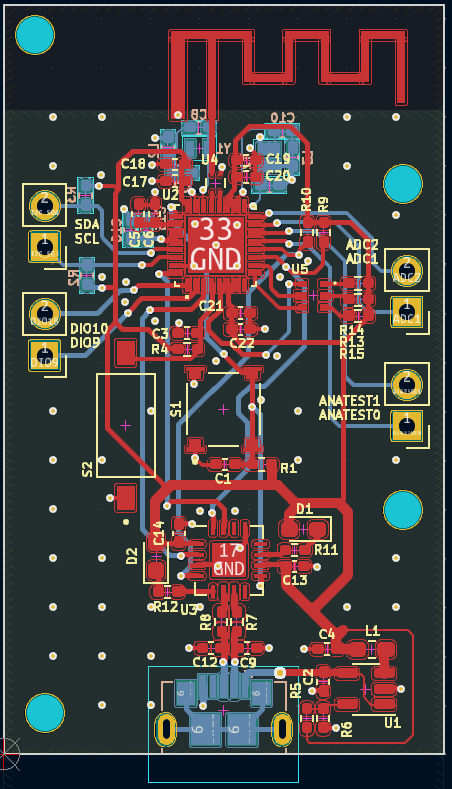
\includegraphics[]{Pics/pcb.png}
\caption{Design of the PCB in KiCad} 
\label{fig:pcb}
\end{figure}

\subsection{Power}
The board is powered by the 5V provided by the USB connector and is stepped down to 3.3V using the TLV62568DBV switching buck regulator in order to power the BlueNRG-2 along with he USB to UART IC. Capacitors were used to filter noise on the 5V and 3.3V lines to provide stable voltage. The TLV62568DBV is adjustable and requires a feedback network in order to maintain the 3.3V output and uses the formula, \[V_{out} = 0.6\left(1 + \frac{R1}{R2}\right)\]. Choosing $R2 = 100k\Omega$, allows us to calculate $R1 = 450k\Omega$. \par

\subsection{Stackup}
The design was implemented on a four layer PCB with the top and bottom layer being the signal and power layers and both middle layers being the ground planes. FR4 is used as the core and prepreg materials and has a dielectric constant of $\epsilon_r = 4.3$ on average. The inner ground planes were stictched with vias for proper grounding along with RF shielding in mind. Using the formula, \[d = \frac{\lambda}{20} = \frac{c}{20*f*\sqrt{\epsilon_r}}\] the distance between vias came out to be about 3.01mm for proper shielding at 2.4GHz.

\subsection{Antenna}
The antenna design is from \cite{an043} and features a small size 2.4 GHz 50$\Omega$ impedance antenna in the form of a copper trace. Design guidelines were considered in order to properly implement it onto the board. That is, the ground plane is voided and the feed point protrudes 0.5mm into the ground plane as shown in Figure~\ref{fig:ant}. There is also a via to ground to supply the return path.

\begin{figure}[H]
\centering
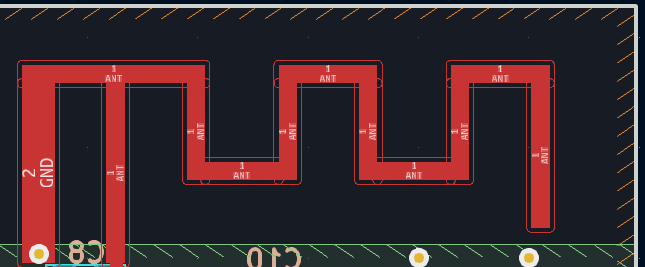
\includegraphics[]{Pics/ant.png}
\caption{Voiding of the ground plane and feed point protruding.} 
\label{fig:ant}
\end{figure}

\subsection{Oscillators}
Crystal oscillators were used in order to generate a stable clock source for the BlueNRG-2. \cite{an2867} was referenced in order to keep the signal-to-noise ratio (SNR) below acceptable limits. The two biggest tips were keeping the crystal as close to the BLUENRG-2 to reduce inducive and capacitive effects as well as keeping any potential high frequency signals away from the oscillator and are shown in \ref{fig:osc}. To achieve this, the oscillator network was placed on the bottom of the board away from the bluetooth antenna traces.

\begin{figure}[H]
\centering
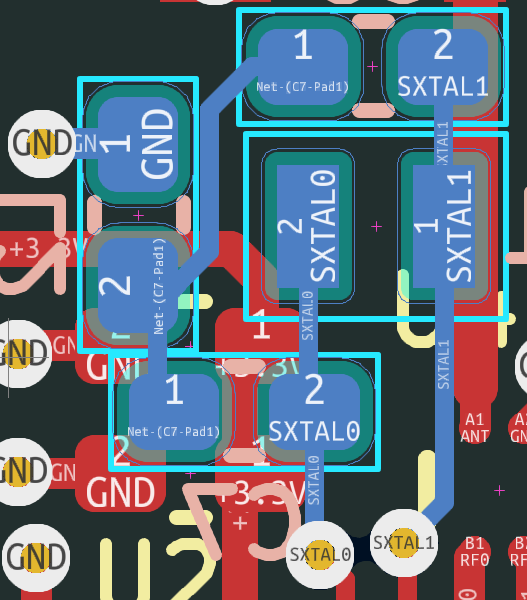
\includegraphics[]{Pics/osc.png}
\caption{Following guidelines listed in \cite{an2867}.} 
\label{fig:osc}
\end{figure}

\section{Software}

\subsection{Simulation}
A simulation of the BlueNRG-2's physical layer was simulated using MATLAB's Bluetooth LE waveform generator app. The generated Bluetooth LE waveforms are visualized in the frequency domain using the spectrum analyzer. The constellation diagram shows all the possible combinations of symbols that can be transmitted by the PHY. The eye diagram helps evaluate the quality of the signal.
\begin{figure}[H]
\centering
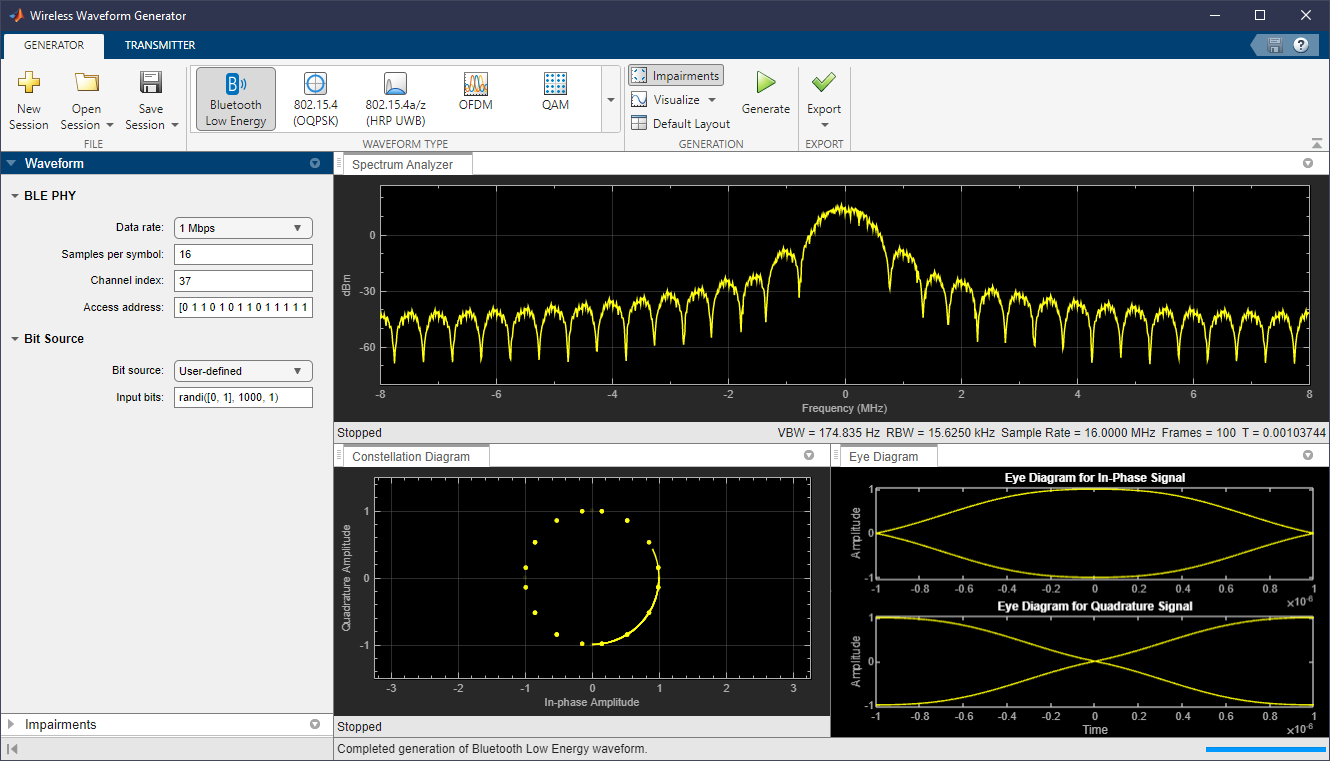
\includegraphics[width=\textwidth]{Pics/blesim.png}
\caption{Simulation of the BlueNRG-2's physical layer generating a waveform.}
\label{fig:ble}
\end{figure}

\subsection{Programming}
Using \cite{pm0257,an4872} as a reference, Communication with the BlueNRG-2 bootloader requires the following UART communication: 8 bit data, no parity bits, a stop bit 1, no flow control, and a baudrate range in the range of 500-460800 bits/s. In order to activate the bootloader, the boot pin on the BlueNRG-2 must be high during a device reset. A toggle switch was implemented to set the boot pin high or low. Next, the STMicroelectronics RF-Flasher utility is used to write and erase the flash memory that stores the firmware. The utility already implements the necessary UART bootloader commands needed to flash the firmware onto the BlueNRG-2. \par
To create firmware for the BlueNRG-2, C/C++ will be written and compiled along with the libraries associated with the transmitter and needed to generate the binaries that will be flashed onto the device. The libaries contain APIS via the hardware abstraction layer that can be used to access registers and read and write to them.
\section{Conclusion}
While the PCB was successfully created in ECAD software and all the design requirements were met, the board was unable to be manufactured in time to be tested or programmed. Thus, it is still unknown whether or not the bluetooth capabilities of the board work. It is also unknown if the board is capable of communicating with the computer via UART. However, when the board does arrive and if the UART communication is successful, tests like single tone generation to verify that the frequency contents of the waveform generated is correct and RX tests to calculate the packet error rate will be conducted using the STMicroelectronics BlueNRG GUI software.
\appendices
\section{}
Pseudocode was written and demonstrates how the BlueNRG would react to successful data transfer. The GPIO register description is located in \cite{bluenrg2}.
\begin{lstlisting}
#include "BlueNRG2_it.h"
#include "BlueNRG2_conf.h"
#include "SDK_EVAL_Config.h"
#include "sleep.h"

int main(void) {

        /* System Init */
        SystemInit();
        /* Identify BlueNRG2 platform */
        SdkEvalIdentification();
        /* Configure I/O communication channel */
        SdkEvalComUartInit(UART_BAUDRATE);
        /* BLE stack init */
        HAL_STATUS ret = BlueNRG_Stack_Initialization(&BlueNRG_Stack_Init_params);
        if (ret != BLE_STATUS_SUCCESS) {
                printf("Error in BlueNRG_Stack_Initialization() 0x%02x\r\n", ret);
                while(1);
        }
        /* Device Initialization: BLE stack GATT and GAP Init APIs.
        It could add BLE services and characteristics (if it is a GATT
        server) and initialize its state machine and other specific drivers
        (i.e. leds, buttons, sensors, ...) */
        ret = DeviceInit();
        if (ret != BLE_STATUS_SUCCESS) {
                /* Device failed to initialize
                   Turn on RED LED and hang*/
                BlueNRG->GPIO_BASE_ADDR->DATA |= BIT_DIO2; // Red
                while (1);
        }
        while(1) {
                /* BLE Stack Tick 
                   returns BLE_STATUS_SUCCESS if a user is connected */
                ret = BTLE_StackTick();
                /* Application Tick: user application where application state machine
                is handled */
                if (ret != BLE_STATUS_SUCCESS) {
                        /* Turn on RED LED */
                        BlueNRG->GPIO_BASE_ADDR->DATA |= BIT_DIO2; // Red
                }
                else {
                /* Application Tick: user application where application state machine
                is handled */
                        APP_Tick();
                }
                /* Power Save management: enable sleep mode with wakeup on radio
                operating timings (adverting, connections intervals) */
                BlueNRG_Sleep(SLEEPMODE_WAKETIMER, 0, 0, 0);
        }/* while (1) */
} /* end main() */

/* Demo the red blue and green LEDs blinking in 1 second intervals */
void APP_Tick() {
        /* Blink RGB in order */
        BlueNRG->GPIO_BASE_ADDR->DATA |= BIT_DIO2; //Red
        HAL_DELAY(1000);
        BlueNRG->GPIO_BASE_ADDR->DATA |= BIT_DIO3; //Green
        HAL_DELAY(1000);
        BlueNRG->GPIO_BASE_ADDR->DATA |= BIT_DIO6; //Blue
        HAL_DELAY(1000);

        /* Turn off RGB in order */
        BlueNRG->GPIO_BASE_ADDR->DATA &= !BIT_DIO2; //Red
        HAL_DELAY(1000);
        BlueNRG->GPIO_BASE_ADDR->DATA &= !BIT_DIO3;//Green
        HAL_DELAY(1000);
        BlueNRG->GPIO_BASE_ADDR->DATA &= !BIT_DIO6;//Blue
        HAL_DELAY(1000);
}
\end{lstlisting}
\begin{figure}[!ht]
\caption{Main code that blinks RGB LEDs every second when a bluetooth connection is successfully established.}
\label{appendix:code}
\end{figure}

%\end{comment}
%\section*{Acknowledgment}
%This work is supported by the Center for Energy and Geo Processing at Georgia Institute of Technology and King Fahd University of Petroleum and Minerals (KFUPM), under research grant number GTEC1601.
%The authors appreciate KFUPM support of this work

%\newpage
%\setstretch{1.28}
\bibliographystyle{IEEEtran}
\bibliography{IEEEabrv,Ref}

% biography section
% 
% If you have an EPS/PDF photo (graphicx package needed) extra braces are
% needed around the contents of the optional argument to biography to prevent
% the LaTeX parser from getting confused when it sees the complicated
% \includegraphics command within an optional argument. (You could create
% your own custom macro containing the \includegraphics command to make things
% simpler here.)

\end{document}
